\chapter{全纯开拓\label{chap6}}
设$f$是域$G$上的一个全纯函数,如果存在一个比$G$更大的域$D$($D\supset G,D\ne G$)以及$D$上的全纯函数$F$,使得当$z\in G$时有$F(z)=f(z)$,就说$F$是$f$在域$D$上的\textbf{全纯开拓}.
\index{Q!全纯开拓}

例如,函数$f(z)=\sum_{n=0}^\infty z^n$是域$G=\{z:|z|<1\}$上的全纯函数,令$D=\MC\backslash\{1\}$,则$F(z)=\frac1{1-z}$是$D$上的全纯函数.显然$D\supset G$,
且当$z\in G$时有$F(z)=f(z)$,所以$F$是$f$在$D$上的全纯开拓.

设$F$是$f$在$D$上的一个全纯开拓,如果$F_1$是$f$在$D$上的另一个全纯开拓,由于当$z\in G$时有
\[F(z)=f(z)=F_1(z),\]
故由唯一性定理,当$z\in D$时,$F(z)=F_1(z)$.这说明,如果存在全纯开拓,那么这个开拓是唯一的.
对于给定的域$G$及$f\in H(G)$,是否一定能将$f$全纯开拓到比$G$更大的域上去呢?答案是否定的.例如,单位圆盘$B(0,1)$上的全纯函数
\[f(z)=\sum_{n=0}^\infty z^{n!}\]
就不能全纯开拓到比$B(0,1)$更大的域上去.我们将在例 \ref{exam6.2.5} 中给出这一事实的证明.

如果$f\in H(G)$能全纯开拓,那么如何开拓呢?在这一章中,我们将介绍两种全纯开拓的方法:用Schwarz对称原理和用幂级数进行全纯开拓.

\section{Schwarz对称原理\label{sec6.1}}
先证明下面的Painlev\'e连续开拓原理:
\begin{theorem}[(\textbf{Painlev\'e原理})]\label{thm6.1.1}\index{D!定理!Painlev\'e原理}
设$D$是域,$\gamma_1,\cdots,\gamma_n$是$\MC$中的$n$条可求长曲线.如果$f$在$D$上连续,在开集$D\backslash\big(\bigcup_{k=1}^n\gamma_k\big)$上全纯,那么$f$必在$D$上全纯.
\end{theorem}
\begin{proof}
任取圆盘$B(a,r)\subset D$,只须证明$f$在$B(a,r)$上全纯即可.由Morera定理,只须证明对$B(a,r)$中任意可求长简单闭曲线$l$,总有
\begin{equation}\label{eq6.1.1}
\int\limits_lf(z)\dz=0
\end{equation}
就行了. 如果$l$不与$\gamma_1,\cdots,\gamma_n$中的任意一条相交,\eqref{eq6.1.1} 式当然成立。今设$l$与$\gamma_k$相交,那么由Cauchy积分定理(定理 \ref{thm3.2.4}),只要将$f$沿$l$的积分分解成沿图 \ref{fig6.1} 中箭头方向所表示的两条闭曲线的积分,便知 \eqref{eq6.1.1} 式也成立.这里考虑的是最简单的情形,一般情形的证明完全类似.
\begin{figure}[!ht]
\centering
\begin{tikzpicture}[thick,every node/.style={inner sep=2pt},
>={Stealth[width=3pt]}]
\draw(0,0)circle(2);
\draw(-140:3.7)node[right]{$\gamma_k$}[bend left=30]to(0,-0.3)
[bend right=35]to(2.2,1.9);
\fill(-140:3.7)circle(1pt);
\draw(-130:1.7)arc(-130:-30:0.4)[bend left=40]to(-40:1.4)node[below left]{$l$}arc
(-120:0:0.3)[bend right=17]to(40:1.5)arc(40:140:0.3)[bend left=30]
to(130:0.7)[bend right=40]to(170:1.2)[bend right=33]to(-130:1.7)--cycle;
\draw[->,very thin](-40:1.4)--++(-25:0.1);
\draw[->,very thin](0,0.53)--++(-170:0.1);
\draw[->](-0.2,-0.2)[bend right=5]to(0.3,-0.1);
\draw[<-,yshift=-0.25cm](-0.2,-0.2)[bend right=5]to(0.3,-0.1);
\node at(0,-2.25){$B(a,r)$};
\end{tikzpicture}
\caption{\label{fig6.1}}
\end{figure}
\end{proof}

利用Painlev\'e原理,即可证明下面的Schwarz对称原理:
\begin{theorem}[(\textbf{Schwarz对称原理})]\label{thm6.1.2}\index{D!定理!Schwarz对称原理}
设域$D$关于实轴对称,如果$f$满足
\begin{eenum}
  \item \label{thm6.1.2.1} $f$在$D\cap\{z\in\MC:\Im z>0\}$上全纯;
  \item \label{thm6.1.2.2} $f$在$D\cap\{z\in\MC:\Im z\ge0\}$上连续;
  \item \label{thm6.1.2.3} $f(D\cap\MR)\subset\MR$,
\end{eenum}
那么
\[F(z)=\begin{cases}
f(z),&z\in D\cap\{z\in \MC:\Im z\ge0\};\\
\bar{f(\bar z)},&z\in D\cap \{z\in\MC:\Im z<0\}
\end{cases}\]
便是$f$在$D$上的全纯开拓.
\end{theorem}
\begin{proof}
我们证明$F\in H(D)$. 显然,$F$在$D\cap\{z\in\MC:\Im z>0\}$中是全纯的. 今任取$z\in D\cap\{z\in\MC:\Im z<0\}$,那么$\zeta=\bar z\in D\cap\{z\in\MC:\Im z>0\}$,于是
\[\pp{}{\bar z}F(z)=\pp{}{\bar z}\bar{f(\bar z)}=\bar{\pp{}zf(\bar z)}
=\bar{\pp{}{\bar\zeta}f(\zeta)}=0.\]
这就证明了$F$在$D\cap\{z\in\MC:\Im z<0\}$上全纯. 今任取$x_0\in D\cap\MR$,由 \ref{thm6.1.2.3},$f(z_0)$取实数值,因而当$z$在$D$的下半平面部分趋于$x_0$时,有
\[\lim_{z\to x_0}F(z)=\lim_{\bar z\to x_0}\bar{f(\bar z)}=\bar{f(x_0)}
=f(x_0)=F(x_0),\]
故$F$在$D$上连续.由Painlev\'e原理即知$F\in H(D)$.
\end{proof}

Schwarz对称原理可以推广到更一般的情形.为了叙述方便,对$\MC_\infty$中的圆周$\gamma$分别用$\MC_\infty^+(\gamma)$和$\MC_\infty^-(\gamma)$表示$\MC_\infty$被$\gamma$分成的两个单连通域.实际上,$\MC_\infty^+(\gamma)$和$\MC_\infty^-(\gamma)$就是圆周$\gamma$的两侧.
\begin{theorem}[(\textbf{推广的Schwarz对称原理})]\label{thm6.1.3}\index{D!定理!推广的Schwarz对称原理}
设$\MC_\infty$中的域$D$关于圆周$\gamma=\{z\in\MC:|z-z_0|=r\}$对称,如果$f$满足
\begin{eenum}
  \item \label{thm6.1.3.1}$f$在$D\cap\MC_\infty^+(\gamma)$上全纯;
  \item \label{thm6.1.3.2}$f$在$D\cap\big(\MC_\infty^+(\gamma)\cup\gamma\big)$上连续;
  \item \label{thm6.1.3.3}$f(D\cap\gamma)\subset\Gamma$,这里,$\Gamma=\{w\in\MC:|w-w_0|=\rho\}$是一个圆周;
  \item \label{thm6.1.3.4}对于任意$z\in D\cap\MC_\infty^+(\gamma),f(z)\ne w_0$,
\end{eenum}
那么$f$能全纯开拓到$D$上,成为$D$上的全纯函数$F$,$F$将$D$中关于$\gamma$对称的两点映为$F(D)$中关于$\Gamma$对称的两点.
\end{theorem}
\begin{proof}
  由第 \ref{chap2} 章 \ref{sec2.5} 节知道,$z$与$z_0+\frac{r^2}{\bar z-\bar {z_0}}$关于圆周$\gamma$对称,$w$与$w_0+\frac{\rho^2}{\bar w-\bar {w_0}}$关于圆周$\Gamma$对称. 令
  \[F(z)=\begin{cases}
  f(z),&z\in D\cap\big(\MC_\infty^+(\gamma)\cup\gamma\big);\\
  w_0+\frac{\rho^2}{\bar{f\big(z_0+\frac{r^2}{\bar z-\bar a}\big)}-\bar w_0},&z\in D\cap
  \MC_\infty^-(\gamma),
  \end{cases}\]
由定义,$F$在$D\cap\MC_\infty^+(\gamma)$中全纯;用定理 \ref{thm6.1.2} 证明中的方法即知$F$也在$D\cap\MC_\infty^-(\gamma)$中全纯,这里用到了条件 \ref{thm6.1.3.4}. 现在证明$F$在$D$上连续.为此任取$\zeta\in D\cap\gamma$,当$z\in D\cap\MC_\infty^-(\gamma)$,且$z\to\zeta$时,总有$z_0+\frac{r^2}{\bar z-\bar a}\in D\cap\MC_\infty^+(\gamma)$,且$z_0+\frac{r^2}{\bar z-\bar a}\to\zeta$. 因而 $f\bigg(z_0+\frac{r^2}{\bar z-\bar a}\bigg)\to f(\zeta)\in\Gamma$,于是也有$  w_0+\frac{\rho^2}{\bar{f\big(z_0+\frac{r^2}{\bar z-\bar a}\big)}-\bar w_0}\to f(\zeta)$,即$F(z)\to f(\zeta)$.这就证明了$F\in C(D)$.于是由Painlev\'e原理即知$F\in H(D)$.
\end{proof}

注意,在上面的证明中,我们假定$\gamma$和$\Gamma$都是$\MC$中的圆周.实际上,$\gamma$和$\Gamma$中有一条(或者两条)是直线,定理当然也成立.特别地,当$\gamma$和$\Gamma$都是实轴时,就得到定理 \ref{thm6.1.2}.

有时,下面这种特殊情形的Schwarz对称原理很有用处,它是定理 \ref{thm6.1.3} 的一个推论.
\begin{theorem}[(\textbf{双全纯映射的 Schwarz对称原理})]\label{thm6.1.4}
\index{D!定理!双全纯映射的 Schwarz对称原理}
设$\MC_\infty$中的域$D$关于圆周$\gamma=\{z\in\MC:|z-z_0|=r\}$对称,如果$f$满足
\begin{eenum}
  \item $f$在$D\cap\MC_\infty^+(\gamma)$上单叶全纯;
  \item $f$在$D\cap\big(\MC_\infty^+(\gamma)\cup\gamma\big)$上单叶连续;
  \item $f(D\cap\gamma)\subset\Gamma$,这里,$\Gamma=\{w\in\MC:|w-w_0|=\rho\}$是一个圆周;
  \item 对于任意$z\in D\cap\MC_\infty^+(\gamma),f(z)\ne w_0$,
\end{eenum}
那么$f$能全纯开拓到$D$上,成为$D$上的单叶全纯函数$F$,$F$将$D$中关于$\gamma$对称的两点映为$F(D)$中关于$\Gamma$对称的两点.
\end{theorem}

下面看两个用Schwarz对称原理来构造双全纯映射的例子.
\begin{example}\label{exam6.1.5}
设$0<a<\infty,L_k=\bigg\{z=k\pi+\frac\pi2+\ii y:0\le y\le a\bigg\},D=\{z\in\MC:\Im z>0\}\backslash\big(\bigcup_{k=-\infty}^\infty L_k\big)$(图 \ref{fig6.2}),求一双全纯映射,把$D$映为上半平面.
\end{example}
\begin{figure}[!ht]
\centering
\begin{tikzpicture}[thick,every node/.style={inner sep=2pt},
>={Stealth[width=3pt]}]
\draw[->](-2*pi,0)--(-3*pi/2,0)node[below]{$-\pi-\frac\pi2$}
--(-pi/2,0)node[below]{$-\frac\pi2$}--(0,0)node[below]{$O$}
--(pi/2,0)node[below]{$\frac\pi2$}--(3*pi/2,0)node[below]{$\pi+\frac\pi2$}
--(2*pi,0)node[below]{$x$};
\draw[->](0,0)--(0,3*pi/2)node[right]{$y$};
\foreach \x/\y in {{pi/2}/2.8,{-pi/2}/2.8,{-3*pi/2}/2.8,{3*pi/2}/2.8}
{\fill(\x,\y)circle(1pt);\draw(\x,\y)--++(0,-2.8);}
\draw(-pi/2,2.8)node[above]{$-\frac\pi2+a\textrm i$}
(pi/2,2.8)node[above]{$\frac\pi2+a\textrm i$};
\end{tikzpicture}
\caption{\label{fig6.2}}
\end{figure}
\begin{solution}
已知$w=\sin z$把半带状域$G=\bigg\{z\in\MC:\Im z>0,-\frac\pi2<\Re z<\frac\pi2\bigg\}$双全纯地映为上半平面,把点$-\frac\pi2+\ii a,-\frac\pi2,\frac\pi2,\frac\pi2+\ii a$分别映为$-\cosh a,-1,1,\cosh a$,因此,$w=\arcsin\frac{\sin z}{\cosh a}$便将$G$双全纯地映为自己. 这时,开射线
\[\bigg\{z=-\frac\pi2+\ii y:a<y<\infty\bigg\}\]
和
\[\bigg\{z=\frac\pi2+\ii y:a<y<\infty\bigg\}\]
分别被映射为开射线
\[\bigg\{z=-\frac\pi2+\ii y:0<y<\infty\bigg\}\]
和
\[\bigg\{z=\frac\pi2+\ii y:0<y<\infty\bigg\}.\]
反复利用双全纯映射的Schwarz对称原理(定理 \ref{thm6.1.4})无穷多次,便可将
\[w=\arcsin\frac{\sin z}{\cosh a}\]
双全纯地开拓到$D$上,成为$D$上的双全纯映射,它把$D$一一地映为上半平面.
\end{solution}

\begin{example}\label{exam6.1.6}
圆环$D=\{z\in\MC:r_1<|z|<r_2\}$与圆环$G=\{w\in\MC:R_1<|w|<R_2\}$双全纯等价的充分必要条件是
\begin{equation}\label{eq6.1.2}
\frac{r_2}{r_1}=\frac{R_2}{R_1}.
\end{equation}
当 \eqref{eq6.1.2} 式成立时,$w=f(z)$是将$D$映为$G$的双全纯映射,当且仅当
\[f(z)=\ee^{\ii\theta}\frac{R_2}{r_2}z,\theta\in\MR\]
或
\[f(z)=\ee^{\ii\theta}\frac{r_1R_2}z,\theta\in\MR.\]
特别地,圆环$D$的全纯自同构群为
\[\Aut(D)=\bigg\{\ee^{\ii\theta}z\text{ 或 }\ee^{\ii\theta}\frac{r_1r_2}z:\theta\in\MR\bigg\}.\]
\end{example}
\begin{proof}
如果 \eqref{eq6.1.2} 式成立,那么
\[f(z)=\ee^{\ii\theta}\frac{R_2}{r_2}z,\theta\in\MR\]
或
\[f(z)=\ee^{\ii\theta}\frac{r_1R_2}z,\theta\in\MR.\]
便把$D$双全纯地映为$G$,因而$D$和$G$全纯等价.

现在证明 \eqref{eq6.1.2} 式是必要的.如果$f$将$D$双全纯地映为$G$,那么由习题 \hyperlink{xiti7.3}{7.3} 的第  \hyperlink{xiti7.3.2}{2} 题,$f$也同胚地将$\bar D$映为$\bar G$.先考虑$f$将$|z|=r_1$和$|z|=r_2$分别映为$|w|=R_1$和$|w|=R_2$的情形.令
\begin{align*}
&D_1=\bigg\{z\in\MC:\frac{r_1^2}{r_2}<|z|<r_1\bigg\},\\
&G_1=\bigg\{w\in\MC:\frac{R_1^2}{R_2}<|w|<R_1\bigg\},
\end{align*}
\begin{figure}[!ht]
\centering
\subcaptionbox{\label{fig6.3a}}[0.48\textwidth]
{
\begin{tikzpicture}[thick,every node/.style={inner sep=2pt},scale=0.7,
>={Stealth[width=3pt]}]
\draw[->](0,0)node[below left]{$O$}--(1,0)node[below right]{$\frac{r_1^2}{r_2}$}
--(2.3,0)node[below right]{$r_1$}--(3.5,0)node[below right]{$r_2$}--(4.5,0);
\foreach \x in {1,2.3,3.5}
{\draw(0,0)circle(\x);}
\foreach \x in {0,1,2.3,3.5}
{\fill(\x,0)circle(1.4pt);}
\draw(70:1.9)node{$D_1$}(60:3.1)node{$D$};
\end{tikzpicture}
}
\subcaptionbox{\label{fig6.3b}}[0.48\textwidth]
{
\begin{tikzpicture}[thick,every node/.style={inner sep=2pt},scale=0.8,
>={Stealth[width=3pt]}]
\draw[->](0,0)node[below left]{$O$}--(1,0)node[below right]{$\frac{R_1^2}{R_2}$}
--(2.3,0)node[below right]{$R_1$}--(3.5,0)node[below right]{$R_2$}--(4.5,0);
\foreach \x in {1,2.3,3.5}
{\draw(0,0)circle(\x);}
\foreach \x in {0,1,2.3,3.5}
{\fill(\x,0)circle(1.2pt);}
\draw(70:1.9)node{$G_1$}(60:3.1)node{$G$};
\end{tikzpicture}
}
\caption{\label{fig6.3}}
\end{figure}
那么$D_1$和$G_1$分别是$D$和$G$关于$|z|=r_1$和$|w|=R_1$对称的圆环(图 \ref{fig6.3}).根据Schwarz对称原理(定理 \ref{thm6.1.4}),$f$可双全纯开拓到$D_1$上,成为$D\cup D_1\cup\{z\in\MC:|z|=r_1\}$上的双全纯函数,而且$f\big(D\cup D_1\cup\{z\in\MC:|z|=r_1\}\big)=G\cup G_1\cup\{w\in\MC:|w|=R_1\}$.这个过程可继续进行,于是$f$可双全纯开拓到$B(0,r_2)$,成为$B(0,r_2)$上的双全纯映射,而且$f\big(B(0,r_2)\big)
=B(0,R_2),f(0)=0$,因而有$f(z)=\ee^{\ii\theta}\frac{R_2}{r_2}z$.由于同时成立$f\big(B(0,r_1)\big)=B(0,R_1)$,所以也有$f(z)=\ee^{\ii\theta}\frac{R_1}{r_1}z$.由此即得
\[\frac{r_2}{r_1}=\frac{R_2}{R_1}.\]

再考虑$f$将$|z|=r_1$和$|z|=r_2$分别映为$|w|=R_2$和$|w|=R_1$的情形. 这时,$g(z)=\frac{R_1R_2}{f(z)}$也将$D$双全纯地映为$G$,并且将$|z|=r_1$和$|z|=r_2$分别映为$|w|=R_1$和$|w|=R_2$. 由上面的证明便知$\frac{r_2}{r_1}=\frac{R_2}{R_1}$,而且$g(z)=\ee^{\ii\theta}\frac{R_1}{r_1}z$,因而$f(z)=\ee^{-\ii\theta}\frac{r_1R_2}{z}$.
\end{proof}
\begin{xiti}\hypertarget{xiti6.1}{}
\item 设域$D$关于$x$轴对称,$f$在$D$上亚纯,$f(D\cap\MR)\subset\MR\cup\{\infty\}$. 证明:若$z_0\in D$是$f$的极点,则$\bar{z_0}$也是$f$的极点,并且
    \[\Res(f,\bar{z_0})=\bar{\Res(f,z_0)}.\]
\item 设域$D$关于圆周$\partial B(a,r)$对称,$f$在$D$上亚纯,$f\big(D\cap\partial
B(a,r)\big)\subset\partial B(A,R)$.证明:若$z_0,w_0\in D$关于$\partial B(a,r)$对称,$z_0$是$f(z)-A$的$1$阶零点,则$w_0$是$f$的$1$阶极点,并且
\[\Res(f,w_0)=-\frac{R^2(w_0-a)^2}{r^2\bar{f'(z_0)}}.\]
\item 设$0<r<R<\infty,f$在$B(0,R)\backslash\bar{B(0,r)}$上全纯,在$B(0,R)\backslash B(0,r)$上连续.证明:若$f$在$\partial B(0,r)$上恒为零,则在$B(0,R)\backslash\bar{B(0,r)}$上也恒为零.
\item 设$\gamma$是圆周$\partial B(a,R)$上的一段开圆弧.证明:若$f$在$B(a,R)$上全纯,在$B(a,R)\cup\gamma$上连续,并且在$\gamma$上恒为零,则$f$在$B(a,R)$上也恒为零.
\item 将如图 \ref{fig6.4} 所示的单连通域$D$双全纯地映为上半平面.
\begin{figure}[!ht]
\centering
\begin{tikzpicture}[thick,every node/.style={inner sep=2pt},
>={Stealth[width=3pt]}]
\clip(-2,-1.5)rectangle(6,1.5);
\foreach \x in {-2,-1.5,...,10}
\draw[help lines](\x,1.5)--++(-135:5);
\fill[white](-1.1,0.1)--(-0.1,0.1)--(-0.1,1.1)--(0.1,1.1)--(0.1,0.1)--(5.6,0.1)
--(5.6,-0.1)--(0.1,-0.1)--(0.1,-1.1)--(-0.1,-1.1)--(-0.1,-0.1)--(-1.1,-0.1)--cycle;
\draw[->](-1,0)node[below]{$-\textrm i$}--(0,0)node[below left]{$O$}--(5,0);
\draw(4.8,0)--(5.5,0);
\draw(0,-1)node[below]{$-\textrm i$}--(0,1)node[above]{$\textrm i$}
(1,1)node{$D$};
\fill(0,-1)circle(1pt)(0,1)circle(1pt)(-1,0)circle(1pt);
\end{tikzpicture}
\caption{\label{fig6.4}}
\end{figure}
\item 利用Schwarz对称原理证明:若$f$双全纯地将$B(a,r)$映为$B(A,R)$,同胚地将$\bar{B(a,r)}$映为$\bar{B(A,R)}$,则$f$必是分式线性变换.
\item 设$P(x_1,x_2,\cdots,x_n)$是关于$x_1,x_2,\cdots,x_n$的多项式,$f\in H\big(B(0,r)\big),\rho>1$. 证明:若在圆盘$B(0,r)$上成立$f(z)=P\bigg(
    f\bigg(\frac z\rho\bigg),f'\bigg(\frac z\rho\bigg),\cdots,
    f^{(n-1)}\bigg(\frac z\rho\bigg)\bigg)$,则$f$必能全纯开拓到$\MC$.
\item 将如图 \ref{fig6.5} 所示的单连通域$D=\big(\MC\backslash[2,\infty)\big)\backslash
\big(\bar{B(1,1)}\cup\bar{B(-1,1)}\big)$双全纯地映为上半平面.
\begin{figure}[!ht]
\centering
\begin{tikzpicture}[thick,every node/.style={inner sep=2pt},
>={Stealth[width=3pt]}]
\clip(-4,-1.5)rectangle(7,1.5);
\foreach \x in {-4,-3.5,...,10}
\draw[help lines](\x,1.5)--++(-135:5);
\fill[white](-1,0)circle(1.1)(1,0)circle(1.1);
\fill[white](1.9,0.1)--(5.3,0.1)--(5.3,-0.1)--(1.9,-0.1)--cycle;
\draw(-2,0)node[below left]{$-2$}(-1,0)node[below]{$-1$};
\draw(0,0)node[below right]{$O$}(1,0)node[below]{$1$}(2,0)node[below right]{$2$};
\draw(5,0)--(5.5,0);
\foreach \x in {-2,-1,0,1,2}
\fill(\x,0)circle(1pt);
\draw(-1,0)circle(1)(1,0)circle(1)(2.5,1)node{$D$};
\draw[->](2,0)--(5.2,0);
\end{tikzpicture}
\caption{\label{fig6.5}}
\end{figure}
\item 设$0<a<\infty,L_k=\bigg\{z=k\pi+\frac\pi2+\ii y,-a\le y\le a\bigg\},D=
\bigg(\MC\backslash\bigg(\bigg(-\infty,-\frac\pi2\bigg]
\cup\bigg[\frac\pi2,\infty\bigg)\bigg)\bigg)\backslash
\big(\bigcup_{k=-\infty}^\infty L_k\big)$是如图 \ref{fig6.6} 所示的单连通域,将$D$双全纯地映为上半平面.
\begin{figure}[!ht]
\centering
\begin{tikzpicture}[thick,every node/.style={inner sep=2pt},xscale=0.6,
>={Stealth[width=3pt]}]
\clip(-10,-2)rectangle(10,2);
\foreach \x in{-10,-9,...,16}
\draw[help lines](\x,2)--++(-148:10);
\fill[white](-9.1,0.1)--(-4.81,0.1)--(-4.81,1.4)--(-4.61,1.4)
--(-4.61,0.1)--(-1.67,0.1)--(-1.67,1.4)--(-1.47,1.4)--(-1.47,-1.4)
--(-1.67,-1.4)--(-1.67,-0.1)--(-4.61,-0.1)--(-4.61,-1.4)--(-4.81,-1.4)
--(-4.81,-0.1)--(-9.1,-0.1)--cycle;
\fill[xscale=-1,white](-9.1,0.1)--(-4.81,0.1)--(-4.81,1.4)--(-4.61,1.4)
--(-4.61,0.1)--(-1.67,0.1)--(-1.67,1.4)--(-1.47,1.4)--(-1.47,-1.4)
--(-1.67,-1.4)--(-1.67,-0.1)--(-4.61,-0.1)--(-4.61,-1.4)--(-4.81,-1.4)
--(-4.81,-0.1)--(-9.1,-0.1)--cycle;

\draw[->,yscale=1.3](-pi/2,1)--(-pi/2,-1)(-3*pi/2,1)--(-3*pi/2,-1)
(pi/2,1)--(pi/2,-1)(3*pi/2,1)--(3*pi/2,-1)(-pi/2,0)--(-9,0)
(pi/2,0)--(8.7,0);
\draw(8.6,0)--(9,0);
\draw(-3*pi/2,0)node[below left]{$-\frac{3\pi}2$}
(-pi/2,0)node[below left]{$-\frac\pi2$}(pi/2,0)node[below right]{$\frac\pi2$}
(3*pi/2,0)node[below right]{$\frac{3\pi}2$}(0,0.6)node{$D$};
\foreach \x in {-3*pi/2,-pi/2,pi/2,3*pi/2}
\foreach \y in {1.3,-1.3}
\fill(\x,\y)circle(1.67pt and 1pt);
\end{tikzpicture}
\caption{\label{fig6.6}}
\end{figure}
\item 设$L_k=\{z=k\pi+\ii y:0\le y<\infty\},D=\MC\backslash\big(\operatorname
*{\cup}_{k=-\infty}^\infty L_k\big)$是如图 \ref{fig6.7} 所示的单连通域,将$D$双全纯地映为上半平面.
\begin{figure}[!ht]
\centering
\begin{tikzpicture}[thick,every node/.style={inner sep=2pt},xscale=0.6,
>={Stealth[width=3pt]}]
\clip(-10,-1)rectangle(10,3);
\foreach \x in {-10,-9,...,16}
\draw[help lines](\x,3)--++(-148:10);
\foreach \x in {-2*pi,-pi,0,pi,2*pi}
{\fill[white](\x+0.1,-0.1)--(\x+0.1,2.4)--(\x-0.1,2.4)--(\x,-0.1)--cycle;
\fill(\x,0)circle(1.67pt and 1pt);}
\draw(-2*pi,0)node[below]{$-2\pi$}--(-2*pi,2.4)(-pi,0)node[below]{$-\pi$}--
(-pi,2.4)(0,0)node[below]{$O$}--(0,2.4)(pi,0)node[below]{$\pi$}--(pi,2.4)
(2*pi,0)node[below]{$2\pi$}--(2*pi,2.4)(-1,1.2)node{$D$};
\end{tikzpicture}
\caption{\label{fig6.7}}
\end{figure}
\begin{figure}[!ht]
\centering
\begin{tikzpicture}[thick,every node/.style={inner sep=2pt}]
\tkzInit[xmin=-3.2,xmax=0.53,ymin=-3.25,ymax=0.37]
\tkzClip
\tkzDefPoints{0/0/a,1/-8/b,-4.5/0/c}
\tkzInCenter(a,b,c)\tkzGetPoint{I}
\coordinate(A)at($(a)!(I)!(b)$);
\coordinate(B)at($(a)!(I)!(c)$);
\coordinate(C)at($(b)!(I)!(c)$);
\tkzCalcLength(I,A)\tkzGetLength{IA}
\fill[pattern=north east lines](I)circle(\IA pt);
\tkzCalcLength(a,A)\tkzGetLength{aA}
\fill[white](a)circle(\aA pt);
\fill[white](b)circle(6.64);
\fill[white](c)circle(3.07);

\tkzDrawCircle[thick,color=black](I,A)
\tkzDrawArc[thick,color=black](a,B)(A)
\tkzDrawArc[thick,color=black](c,C)(B)
\tkzDrawArc[thick,color=black](b,A)(C)
\draw(I)node[above,fill=white,inner sep=0pt]{$D$}
(A)node[right]{$A$}(B)node[above]{$B$}(C)node[below left]{$C$};

\end{tikzpicture}
\caption{\label{fig6.8}}
\end{figure}
\item \hypertarget{xiti6.1.11}{} 设$D$是由$3$条与$\partial B(0,1)$正交的圆弧所围成的单连通域,如图 \ref{fig6.8} 所示.证明:若$\varphi$双全纯地将$D$映为上半平面$\MC^+=\{z\in\MC:\Im z>0\}$,同胚地将$\bar D$映为$\bar{\MC^+}$,$A,B,C$分别映为$0,1,\infty$,则$\varphi$可全纯开拓到$B(0,1)$,并且$\varphi\big(B(0,1)\big)=\MC\backslash\{0,1\}$.
\end{xiti}

\section{幂级数的全纯开拓\label{sec6.2}}
这一节要讨论由幂级数确定的和函数如何进行全纯开拓.

设幂级数
\begin{equation}\label{eq6.2.1}
f(z)=\sum_{n=0}^\infty a_nz^n
\end{equation}
的收敛半径为$R$,那么$f$是$B(0,R)$中的全纯函数。今在收敛圆周$\partial B(0,R)$上取点$\zeta$,并在半径$O\zeta$上取点$z_0\ne0$,那么$f$在$z_0$处全纯,故在$z_0$的邻域中有幂级数展开式
\begin{equation}\label{eq6.2.2}
f(z)=\sum_{n=0}^\infty\frac{f^{(n)}(z_0)}{n!}(z-z_0)^n.
\end{equation}
设右端幂级数的收敛半径为$\rho$,那么显然有$\rho\ge R-|z_0|$.这时有两种情形:

(1) 如果$\rho>R-|z_0|$,这时幂级数 \eqref{eq6.2.2} 的收敛圆$B(z_0,\rho)$有一部分在圆盘$B(0,R)$的外部(见图 \ref{fig6.9}).设幂级数 \eqref{eq6.2.2} 在$B(z_0,\rho)$中的和函数为$g$,那么当$z\in B(0,R)\cap B(z_0,\rho)$时,$f(z)=g(z)$,这说明$f$被全纯开拓到$B(z_0,\rho)\backslash\big(B(z_0,\rho)\cap B(0,R)\big)$.这时,称$f$可以沿半径$O\zeta$全纯开拓.
\begin{figure}[!ht]
\centering
\begin{minipage}{0.48\linewidth}
\centering
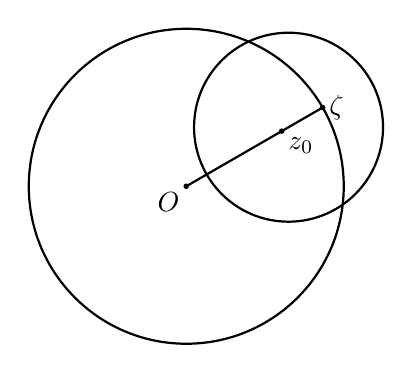
\begin{tikzpicture}[thick,every node/.style={inner sep=2pt}]
\draw(0,0)node[below left]{$O$}circle(2);
\draw(30:1.5)circle(1.2);
\draw(0,0)--(30:1.4)node[below right]{$z_0$}--(30:2)node[right]{$\zeta$};
\fill(0,0)circle(1pt)(30:1.4)circle(1pt)(30:2)circle(1pt);
\end{tikzpicture}
\caption{\label{fig6.9}}
\end{minipage}\hfill
\begin{minipage}{0.48\linewidth}
\centering
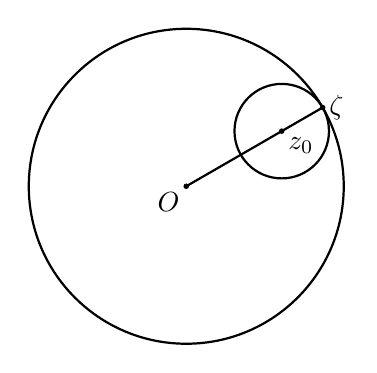
\begin{tikzpicture}[thick,every node/.style={inner sep=2pt}]
\draw(0,0)node[below left]{$O$}circle(2);
\draw(30:1.4)circle(0.6);
\draw(0,0)--(30:1.4)node[below right]{$z_0$}--(30:2)node[right]{$\zeta$};
\fill(0,0)circle(1pt)(30:1.4)circle(1pt)(30:2)circle(1pt);
\end{tikzpicture}
\caption{\label{fig6.10}}
\end{minipage}
\end{figure}

(2) 如果$\rho=R-|z_0|$,这时幂级数 \eqref{eq6.2.2} 的收敛圆$B(z_0,\rho)$含在$B(0,R)$中(图 \ref{fig6.10}),因此$f$不能通过$\zeta$全纯开拓到$B(0,R)$的外部去.也即对$\zeta$的任意邻域$B(\zeta,\delta)$,不存在其上的全纯函数$g$,使得$f(z)=g(z)$在$B(0,R)\cap B(\zeta,\delta)$中成立.这时,称$\zeta$是$f$的一个奇点.

一般来说,我们有下面的
\begin{definition}
设$f$是域$D$上的全纯函数,对于$\zeta\in\partial D$,如果存在$\zeta$的邻域$B(\zeta,\delta)$及其上的全纯函数$g$,使得$f(z)=g(z)$对$z\in D\cap B(\zeta,\delta)$成立,就称$\zeta$是$f$的\textbf{正则点}\index{Z!正则点},否则称$\zeta$为$f$的\textbf{奇点}\index{Q!奇点}.
\end{definition}

\begin{example}\label{exam6.2.2}
幂级数$f(z)=\sum_{n=0}^\infty z^n$的收敛半径$R=1$. 取$z_0\in B(0,1),z_0\ne0$,则$f$在$z_0$处的幂级数展开式为
\[\frac1{1-z}=\frac1{1-z_0}\frac1{1-\frac{z-z_0}{1-z_0}}
=\sum_{n=0}^\infty\frac1{(1-z_0)^{n+1}}(z-z_0)^n.\]
右端幂级数的收敛半径
\[R=\left(\varlimsup_{n\to\infty}\sqrt[\leftroot{-4}\uproot{20}n]{\frac1{|1-z_0|^{n+1}}}
\right)^{-1}=|1-z_0|\ge1-|z_0|,\]
等号成立当且仅当$z_0$是非负实数.这说明除了$z=1$外,$f$都能通过其收敛圆周上的点全纯开拓出去.
\end{example}

上面的例子说明$f$在其收敛圆周上只有一个奇点.那么是否有这样的幂级数,其收敛圆周上一个奇点也没有呢?这是不可能的.
\begin{theorem}\label{thm6.2.3}
幂级数的收敛圆周上必有其奇点.
\end{theorem}
\begin{proof}
设幂级数
\[f(z)=\sum_{n=0}^\infty a_nz^n\]
的收敛半径为$R$($0<R<\infty$),那么$f$是$B(0,R)$中的全纯函数.
如果$\partial B(0,R)$上没有$f$的奇点,那么对每个$\zeta\in\partial(0,R)$,存在$B(\zeta,r_\zeta)$及$B(\zeta,r_\zeta)$上的全纯函数$f_\zeta$,使得当$z\in B(0,R)\cap B(\zeta,r_\zeta)$时,$f(z)=f_\zeta(z)$.显然,$\{B(\zeta,r_\zeta)\}$的全体构成$\partial B(0,R)$的一个开覆盖,由于$\partial B(0,R)$是紧集,故从中可以选出有限个
\[B(\zeta_1,r_{\zeta_1}),\cdots,B(\zeta_m,r_{\zeta_m})\]
使得
\[\partial B(0,R)\subset\bigcup_{n=1}^m B(\zeta_n,r_{\zeta_n}).\]
记
\[D=B(0,R)\cup\big(\bigcup_{n=1}^mB(\zeta_n,r_{\zeta_n})\big),\]
并在$D$上定义函数
\[g(z)=\begin{cases}
f(z),&z\in B(0,R);\\
f_{\zeta_k}(z),&z\in B(\zeta_k,r_{\zeta_k}),k=1,\cdots,m,
\end{cases}\]
则$g$是$D$上的单值全纯函数. 因若$B(\zeta_j,r_{\zeta_j})\cap B(\zeta_k,r_{\zeta_k})
\ne\varnothing$,则当$z\in B(\zeta_j,r_{\zeta_j})\cap B(\zeta_k,r_{\zeta_k})\cap B(0,R)$时,$f_{\zeta_j}(z)=f_{\zeta_k}(z)$.由唯一性定理(定理 \ref{thm4.3.7}),$f_{\zeta_j}$与$f_{\zeta_k}$在$B(\zeta_j,r_{\zeta_j})\cap B(\zeta_k,r_{\zeta_k})$上也相等. 所以,$g$是$f$在$D$上的全纯开拓. 由于
\[g(z)=\sum_{n=0}^\infty \frac{g^{(n)}(0)}{n!}z^n=\sum_{n=0}^\infty
\frac{f^{(n)}(0)}{n!}z^n=\sum_{n=0}^\infty a_nz^n,\]
但它的收敛半径严格大于$R$,这就与假定相矛盾.
\end{proof}

对于给定的幂级数,找出其收敛圆周上的奇点并不是一件容易的事,但对于一些特殊的幂级数,还是可以作出一些判断的.

\begin{prop}\label{prop6.2.4}
设幂级数
\[f(z)=\sum_{n=0}^\infty a_nz^n\]
的收敛半径为$R$($0<R<\infty$),如果存在自然数$n_0$,使得当$n\ge n_0$时总有$a_n\ge0$,那么$z=R$必是$f$的奇点.
\end{prop}
\begin{proof}
如果$z=R$不是$f$的奇点,那么$f$在$\frac R2$处展开的幂级数$\sum_{n=0}^\infty
\frac{f^{(n)}\big(\frac R2\big)}{n!}\bigg(z-\frac R2\bigg)^n$的收敛半径$\rho>\frac R2$,即
\begin{equation}\label{eq6.2.3}
\varlimsup_{n\to\infty}\sqrt[\leftroot{-4}\uproot{20}n]{
\frac{\big|f^{(n)}\big(\frac R2\big)\big|}{n!}}=\frac1\rho<\frac2R.
\end{equation}
由幂级数 \eqref{eq6.2.1} 知
\[f^{(k)}\bigg(\frac R2\bigg)=\sum_{n=k}^\infty n(n-1)\cdots(n-k+1)a_n
\bigg(\frac R2\bigg)^{n-k}.\]
由于当$n\ge n_0$时$a_n\ge0$,故当$k\ge n_0$时,有
\begin{align*}
\bigg|f^{(k)}\bigg(\frac R2\bigg)\bigg|
&=\bigg|\sum_{n=k}^\infty n(n-1)\cdots(n-k+1)a_n\bigg(\frac R2\bigg)^{n-k}\bigg|\\
&=\sum_{n=k}^\infty n(n-1)\cdots(n-k+1)a_n\bigg(\frac R2\bigg)^{n-k}.
\end{align*}
今在收敛圆周$\partial B(0,R)$上任取一点$\ee^{\ii\theta}R$,则当$k\ge n_0$时,有
\begin{equation}\label{eq6.2.4}
\begin{aligned}
\bigg|f^{(k)}\bigg(\frac12\ee^{\ii\theta}R\bigg)\bigg|
&=\bigg|\sum_{n=k}^\infty n(n-1)\cdots(n-k+1)a_n\bigg(\frac {\ee^{\ii\theta}R}2\bigg)^{n-k}\bigg|\\
&\le \sum_{n=k}^\infty n(n-1)\cdots(n-k+1)a_n\bigg(\frac R2\bigg)^{n-k}\\
&=\bigg|f^{(k)}\bigg(\frac R2\bigg)\bigg|.
\end{aligned}
\end{equation}
于是由 \eqref{eq6.2.3} 式和 \eqref{eq6.2.4} 式知道,$f$在$\frac12\ee^{\ii\theta}R$处展开的幂级数
\[\sum_{n=0}^\infty\frac{f^{(n)}\big(\frac12\ee^{\ii\theta}R\big)}{n!}
\bigg(z-\frac12\ee^{\ii\theta}R\bigg)^n\]
的收敛半径为
\[\rho'=\left(\varlimsup_{n\to\infty}
\sqrt[\leftroot{-4}\uproot{20}n]{
\frac{\big|f^{(n)}\big(\frac 12\ee^{\ii\theta}R\big)\big|}{n!}}\right)^{-1}
\ge\left(\varlimsup_{n\to\infty}\sqrt[\leftroot{-4}\uproot{20}n]{
\frac{\big|f^{(n)}\big(\frac R2\big)\big|}{n!}}\right)^{-1}
>\frac R2,\]
这说明$\ee^{\ii\theta}R$是$f$的正则点.由于$\ee^{\ii\theta}R$是$\partial B(0,R)$上的任意点,所以收敛圆周$\partial B(0,R)$上没有$f$的奇点,这与定理 \ref{thm6.2.3} 的结论相矛盾.
\end{proof}

定理 \ref{thm6.2.3} 断言幂级数在其收敛圆周上必有奇点,是否也必有正则点呢?下面的例子给出了否定的答案.
\begin{example}\label{exam6.2.5}
幂级数$f(z)=\sum_{n=0}^\infty z^{n!}$的收敛半径显然为$1$,我们证明收敛圆周$\partial B(0,1)$上的每一点都是它的奇点.这时,我们称$\partial B(0,1)$是$f$的\textbf{自然边界}.
\index{Z!自然边界}
\end{example}
\begin{proof}
由命题 \ref{prop6.2.4} 知道,$z=1$是$f$的奇点. 今取既约分数$\frac pq$($q>0$),令$g(z)=f\big(\ee^{\ii2\pi\frac pq}z\big)$,则
\[g(z)=\sum_{n=0}^\infty \ee^{\ii2\pi\frac pqn!}z^{n!}
=\sum_{n=0}^{q-1}\ee^{\ii2\pi\frac pqn!}z^{n!}+\sum_{n=q}^\infty z^{n!}.\]
仍由命题 \ref{prop6.2.4} 知道,$z=1$是$g$的奇点,因而$z=\ee^{\ii2\pi\frac pq}$是$f$的奇点.现在证明$\partial B(0,1)$上的每一点都是$f$的奇点.如果$\zeta\in\partial B(0,1)$不是$f$的奇点,则必存在圆盘$B(\zeta,r)$,使得$f$能全纯开拓到$B(\zeta,r)$,故$\partial B(0,1)\cap B(\zeta,r)$中的每个点都是$f$的正则点.而$\partial B(0,1)\cap B(\zeta,r)$中必有形如$\ee^{\ii2\pi\frac pq}$的点,这就和上面的结论相矛盾.
\end{proof}

\begin{example}\label{exam6.2.6}
研究幂级数$f(z)=\sum_{n=1}^\infty\frac{z^{n!}}{n^2}$的奇点.
\end{example}
\begin{solution}
上述幂级数的收敛半径显然为$1$,并且在其闭收敛圆盘$\bar{B(0,1)}$上绝对一致收敛.用与例 \ref{exam6.2.5} 完全相同的方法,知其收敛圆周上的每一点都是它的奇点,即单位圆周为其自然边界.
\end{solution}

从例 \ref{exam6.2.2}、例 \ref{exam6.2.5} 和例 \ref{exam6.2.6} 这3个例子来看,幂级数在其收敛圆周上的收敛性质与奇点性质没有必然的联系.

\begin{xiti}
\item 证明:幂级数收敛圆周上的点是否为其和函数的奇点,与该幂级数的前有限项无关.
\item 证明:若幂级数的收敛圆周上有其和函数的极点,则该幂级数在其收敛圆周上处处发散.
\item 证明:若幂级数$\sum_{n=0}^\infty a_nz^n$的和函数在其收敛圆周上有$1$阶极点$z_0$,此外再无其他奇点,则
    \[\lim_{n\to\infty}\frac{a_n}{a_{n+1}}=z_0.\]
\item 设$f(z)=\sum_{n=0}^\infty a_nz^n$的收敛半径为$1$,$F(w)=f\bigg(\frac w{1+w}\bigg)=\sum_{n=0}^\infty b_nw^n$的收敛半径为$\rho$. 证明:
\begin{enuma}
  \item $\rho\ge\frac12$,并且$-1$是$f(z)$的奇点当且仅当$\rho=\frac12$;
  \item 若$\frac12<\rho<1$,则$f(z)$能全纯开拓到$B\bigg(-\frac{\rho^2}{1-\rho^2},\frac{\rho^2}{1-\rho^2}\bigg)$;
  \item 若$\rho=1$,则$f(z)$能全纯开拓到$\bigg\{z\in\MC:\Re z<\frac12\bigg\}$;
  \item 若$\rho>1$,则$f(z)$能全纯开拓到$\MC\backslash\bar{B\bigg(\frac{\rho^2} {\rho^2-1},\frac{\rho}{\rho^2-1}\bigg)}$;
  \item 若$\rho=\infty$,则$f(z)$能全纯开拓到$\MC\backslash\{1\}$.
\end{enuma}
\item 设$D$是域. 证明:存在$f\in H(D)$,使得$\partial D$中的每个点皆是$f$的奇点.
\item 证明:$\sum_{n=0}^\infty z^{2^n}$的收敛圆周上的每个点皆为其和函数的奇点.
\item 证明:$\sum_{n=0}^\infty \frac{z^{2^n}}{2^n}$的收敛圆周上的每个点皆为其和函数的奇点.
\item 设$f(z)=\sum_{n=0}^\infty a_nz^n$的收敛半径为$1$,$a_n$($n\ge0$)是实数,$S_n=\sum_{k=0}^na_k $.证明:若$S_n\to\infty$($n\to\infty$),则$1$是$f(z)$的奇点.举例说明,
    仅仅$|S_n|\to\infty$不能保证$1$是$f(z)$的奇点.\\
(\textbf{提示}:考虑$\frac{f(z)}{1-z}$.)
\item 证明:若幂级数$\sum_{n=0}^\infty a_nz^n$的收敛半径为$1$,其和函数在$\partial B(0,1)$上有$1$阶极点$z_1,z_2,\cdots$,\\$z_m$,此外再无其他奇点,则$\{a_n\}$有界.
\item 设$f(z)=\sum_{n=0}^\infty a_nz^n$的收敛半径为$1$,并且$\lim_{n\to\infty}a_n=0$. 证明:若$z_0\in\partial B(0,1)$不是$f(z)$的奇点,则$\sum_{n=0}^\infty a_nz_0^n$收敛.
\end{xiti}

\section{多值全纯函数与单值性定理\label{sec6.3}}

前面我们已经遇到过为数不少的初等多值全纯函数,产生多值的唯一原因是辐角函数$\Arg z$在$\MC\backslash\{0\}$上不能选出单值的连续分支.因此,若初等多值全纯函数在单连通域上有定义,则必能在这个单连通域上选出单值的全纯分支,这就是所谓的单值性定理.

如何定义多值全纯函数并非易事.本节将利用幂级数沿曲线全纯开拓的概念来定义多值全纯函数,然后证明单值性定理对于多值全纯函数也是成立的.最后,作为单值性定理的一个应用,我们给出Liouville定理的推广——Picard小定理.
\begin{definition}\label{def6.3.1}
设幂级数$P(z)=\sum_{n=0}^\infty a_n(z-a)^n$的收敛半径$R>0,z=\gamma(t)$($\alpha\le t\le \beta$)是以$a$为起点的平面曲线. 若存在幂级数族$P_t(z)=\sum_{n=0}^\infty a_n(t)\big(z-\gamma(t)\big)^n$,它具有下列性质:
\begin{eenum}
  \item 对任意$t\in[\alpha,\beta],P_t$的收敛圆盘$B_t$不退化为一点;
  \item 对任意$t_0\in[\alpha,\beta]$,存在$\delta>0$,当$t\in(t_0-\delta,t_0+\delta)\cap[\alpha,\beta]$时,总有$B_t\cap B_{t_0}\ne\varnothing$,并且$P_t$和$P_{t_0}$在$B_t\cap B_{t_0}$上恒等;
  \item $P_\alpha=P$,
\end{eenum}
则称$P$能沿曲线$\gamma$全纯开拓,并称$P_\beta$是$P$沿曲线$\gamma$的全纯开拓.
\index{Q!全纯开拓!沿曲线全纯开拓}
\end{definition}

\begin{example}\label{exam6.3.2}
设幂级数$P(z)=\sum_{n=0}^\infty a_n(z-a)^n$的收敛半径$R>0$,若$z_0\in\bar{B(0,R)}$不是$P$的奇点,则$P$能沿线段$[a,z_0]$全纯开拓;若$w_0\in\partial B(a,R)$是$P$的奇点,则$P$不能沿半径$[a,w_0]$全纯开拓.
\end{example}

\begin{example}\label{exam6.3.3}
幂级数
\[\log|z|+\ii\arg z=\sum_{n=1}^\infty\frac{(-1)^{n-1}}n(z-1)^n\]
沿$\partial B(0,1)$正向的全纯开拓为
\[\log|z|+\ii(\arg z+2\pi)=2\pi\ii+\sum_{n=1}^\infty\frac{(-1)^{n-1}}n(z-1)^n;\]
沿$\partial B(0,1)$负向的全纯开拓为
\[\log|z|+\ii(\arg z-2\pi)=-2\pi\ii+\sum_{n=1}^\infty\frac{(-1)^{n-1}}n(z-1)^n.\]
这表明幂级数沿具有相同起点和终点的两条不同曲线的全纯开拓可能不同.
\end{example}

\begin{prop}\label{prop6.3.4}
若幂级数能沿某曲线全纯开拓,则它沿该曲线的全纯开拓是唯一的.
\end{prop}
\begin{proof}
设幂级数$P(z)=\sum_{n=0}^\infty a_n(z-a)^n$的收敛半径$R>0$,$z=\gamma(t)$($\alpha\le t\le\beta$)是以$a$为起点的平面曲线,幂级数族$P_t$和$Q_t$给出了$P$沿曲线$\gamma$的两个全纯开拓$P_\beta$和$Q_\beta$,我们的目标是证明$P_\beta=Q_\beta$.

设$P_t$和$Q_t$的收敛圆盘分别为$B_t$和$U_t$,$\Gamma=\{t\in[\alpha,\beta]:P_t=Q_t\}$.首先,可证明$\Gamma$是$[\alpha,\beta]$中的开集.事实上,若$t_0\in\Gamma$,则存在$\delta>0$,当$t\in(t_0-\delta,t_0+\delta)\cap[\alpha,\beta]$时,成立$B_t\cap B_{t_0}\ne\varnothing$,$P_t=P_{t_0}\big|_{B_t\cap B_{t_0}}$和$U_t\cap U_{t_0}\ne\varnothing,Q_t=Q_{t_0}\big|_{U_t\cap U_{t_0}}$,因为$P_{t_0}=Q_{t_0},B_{t_0}=U_{t_0}$,由全纯函数的内部唯一性定理便知$P_t=Q_t$,即$t\in\Gamma$.

其次,可证明$\Gamma$是$[\alpha,\beta]$中的闭集.事实上,若$t_0$是$\Gamma$的极限点,则可取$t\in\gamma$,使得$B_t\cap B_{t_0}\ne\varnothing$,$P_t=P_{t_0}\big|_{B_t\cap B_{t_0}}$和$U_t\cap U_{t_0}\ne\varnothing,Q_t=Q_{t_0}\big|_{U_t\cap U_{t_0}}$.因为$P_t=Q_t,B_t=U_t$,由全纯函数的内部唯一性定理便知$P_{t_0}=Q_{t_0}$,即$t_0\in\Gamma$.

注意到$\Gamma\ne\varnothing$,便知$\Gamma=[\alpha,\beta]$. 因此,$P_\beta=Q_\beta$.
\end{proof}

现在给出域$D$上多值全纯函数的定义.
\begin{definition}\label{def6.3.5}
设$D$是域,$f$是$D$上的多值函数,即对任意$z\in D,f(z)$是一个非空复数集.若存在以$a\in D$为收敛圆心、以$R>0$为收敛半径的幂级数$P_0$,使得
\begin{eenum}
  \item $P_0$能沿$D$中以$a$为起点的任意曲线$\gamma$全纯开拓;
  \item 当$z\in D$时,$f(z)=\{P(t):\mbox{$P$是$P_0$沿$D$中连接$a$和$z$的曲线$\gamma$的全纯开拓}\}$,
\end{eenum}
即$f$这个多值函数是由幂级数$P_0$在$D$上经过全纯开拓得到的,则称$f$是$D$上的\textbf{多值全纯函数}.\index{Q!全纯函数!多值全纯函数}
\end{definition}

下面给出本节的主要定理:
\begin{theorem}[(\textbf{单值性定理})]\label{thm6.3.6}\index{D!定理!多值性定理}
设$f$是域$D$上的多值全纯函数,$z_0\in D,w_0\in f(z_0)$.若$G\subset D$是单连通域,$z_0\in G$,则必能在$G$上选出$f$的一个单值全纯分支$g$,使得$g(z_0)=w_0$,并且$f$可由$\sum_{n=0}^\infty\frac{g^{(n)}(z_0)}{n!}(z-z_0)^n$在$D$上经过全纯开拓得到.
\end{theorem}
\begin{proof}
设$f$是由幂级数$P_0$在$D$上经过全纯开拓得到的,故可取$D$中连接$P_0$的收敛圆心和$z_0$的曲线$\gamma$,使得$P_0$沿$\gamma$的全纯开拓$P$满足$P(z_0)=w_0$.注意,$f$也可由幂级数$P$在$D$上经过全纯开拓而得到.

不妨设$G$异于$\MC$,否则$P$的收敛半径为$\infty$,定理显然成立.由Riemann 映射定理(定理 \ref{thm7.2.1}),存在双全纯映射$\varphi$,使得$\varphi\big(B(0,1)\big)=G,\varphi(0)=z_0$,故$(P\circ\varphi)(\zeta)$在$O$处全纯.因此,$h(\zeta)=\sum_{n=0}^\infty\frac{(P\circ\varphi)^{(n)}(0)}{n!}\zeta^n$的收敛半径$\rho>0$.我们断言,对任意$\zeta_0\in B(0,1)$,$h$能沿$[0,\zeta_0]$全纯开拓.实际上,对于$G$中的曲线$z=\gamma(t)=\varphi(t\zeta_0)$($0\le t\le1$),$P$能沿$\Gamma$全纯开拓.设幂级数族$Q_t$给出了$P$沿$\Gamma$的全纯开拓,则幂级数族$h_t(\zeta)=\sum_{n=0}^\infty\frac{(Q_t\circ\varphi)^{(n)}(t\zeta_0)}{n!}(\zeta-t\zeta_0)^n$便给出了$h$沿$[0,\zeta_0]$的全纯开拓.这表明$\zeta_0$不是$h$的奇点,因此$\rho\ge1$.于是$g=h\circ\varphi^{-1}$在$G$上全纯,并且
\begin{equation*}
P(z)=\sum_{n=0}^\infty\frac{g^{(n)}(z_0)}{n!}(z-z_0)^n.
\end{equation*}
\end{proof}

下面的Picard小定理是Liouville定理的推广:
\begin{theorem}[(\textbf{Picard小定理})]\label{thm6.3.7}\index{D!定理!Picard小定理}
设$f$是整函数,若存在$a,b\in\MC,a\ne b$,使得$f(\MC)\subset\MC\backslash\{a,b\}$,则
$f$是常值函数.
\end{theorem}
\begin{proof}
不妨设$a=0,b=1$,否则考虑$\frac{f(z)-a}{b-a}$.由Riemann映射定理(定理 \ref{thm7.2.1})、边界对应定理(定理 \ref{thm7.3.1})和习题 \hyperlink{xiti6.1}{6.1} 的第 \hyperlink{xiti6.1.11}{11} 题知,存在$B(0,1)$上的全纯函数$\varphi$,使得$\varphi\big(B(0,1)\big)=\MC\backslash\{0,1\}$.再由单值性定理(定理 \ref{thm6.3.6})知,多值全纯函数$\varphi^{-1}\circ f$可在$\MC$上选出一个单值全纯分支$\psi$.由Liouville定理,$\psi$是常值函数,故$f$也是常值函数.
\end{proof}

\begin{xiti}\hypertarget{xiti6.3}{}
\item 设$f$是域$D$上的全纯函数,$z_0\in D$.证明:
\[F(z)=\int_{z_0}^zf(\zeta)\textrm d\zeta\]
是$D$上的多值全纯函数.这里,积分是沿$D$中连接$z_0$和$z$的任意可求长曲线进行的.
\item 证明:若$f$是域$D$上非常数的全纯函数,但不是局部双全纯的,则$f^{-1}$一定不是域$G=f(D)$上的多值全纯函数.
\item \hypertarget{xiti6.3.3}{} 举例说明,存在$B(0,1)$上的局部双全纯映射$f$,使得$f^{-1}$不是域$G=f\big(B(0,1)\big)$上的多值全纯函数.
\item \hypertarget{xiti6.3.4}{} 证明:不存在$B(0,1)$上的局部双全纯映射$f$,使得$f\big(B(0,1)\big)=\MC$,并且$f^{-1}$是$\MC$上的多值全纯函数.
\item 证明:不存在$B(0,1)$上的局部双全纯映射$f$,使得$f\big(B(0,1)\big)=\MC\backslash\{a\}$,并且$f^{-1}$是$\MC\backslash\{a\}$上的多值全纯函数.这里,$a$是$\MC$中的一个固定点.
\item 求
\[f(z)=z^{\frac12}=|z|^{\frac12}\ee^{\ii\frac12\arg z}=1+\sum_{k=1}^\infty
\binom{\frac12}{k}(z-1)^k\]
沿单位圆周$\partial B(0,1)$的正向和反向的全纯开拓.
\item 设幂级数族$\{P_t:\alpha\le t\le\beta\}$给出了沿平面曲线$z=\gamma(t)$($\alpha\le t\le\beta$)的全纯开拓.证明:$P_t$的收敛半径$R(t)$或者在$[\alpha,\beta]$上恒为$\infty$,或者是$[\alpha,\beta]$上的正值连续函数.
\end{xiti} 
